\begin{figure}[htp]
\centering
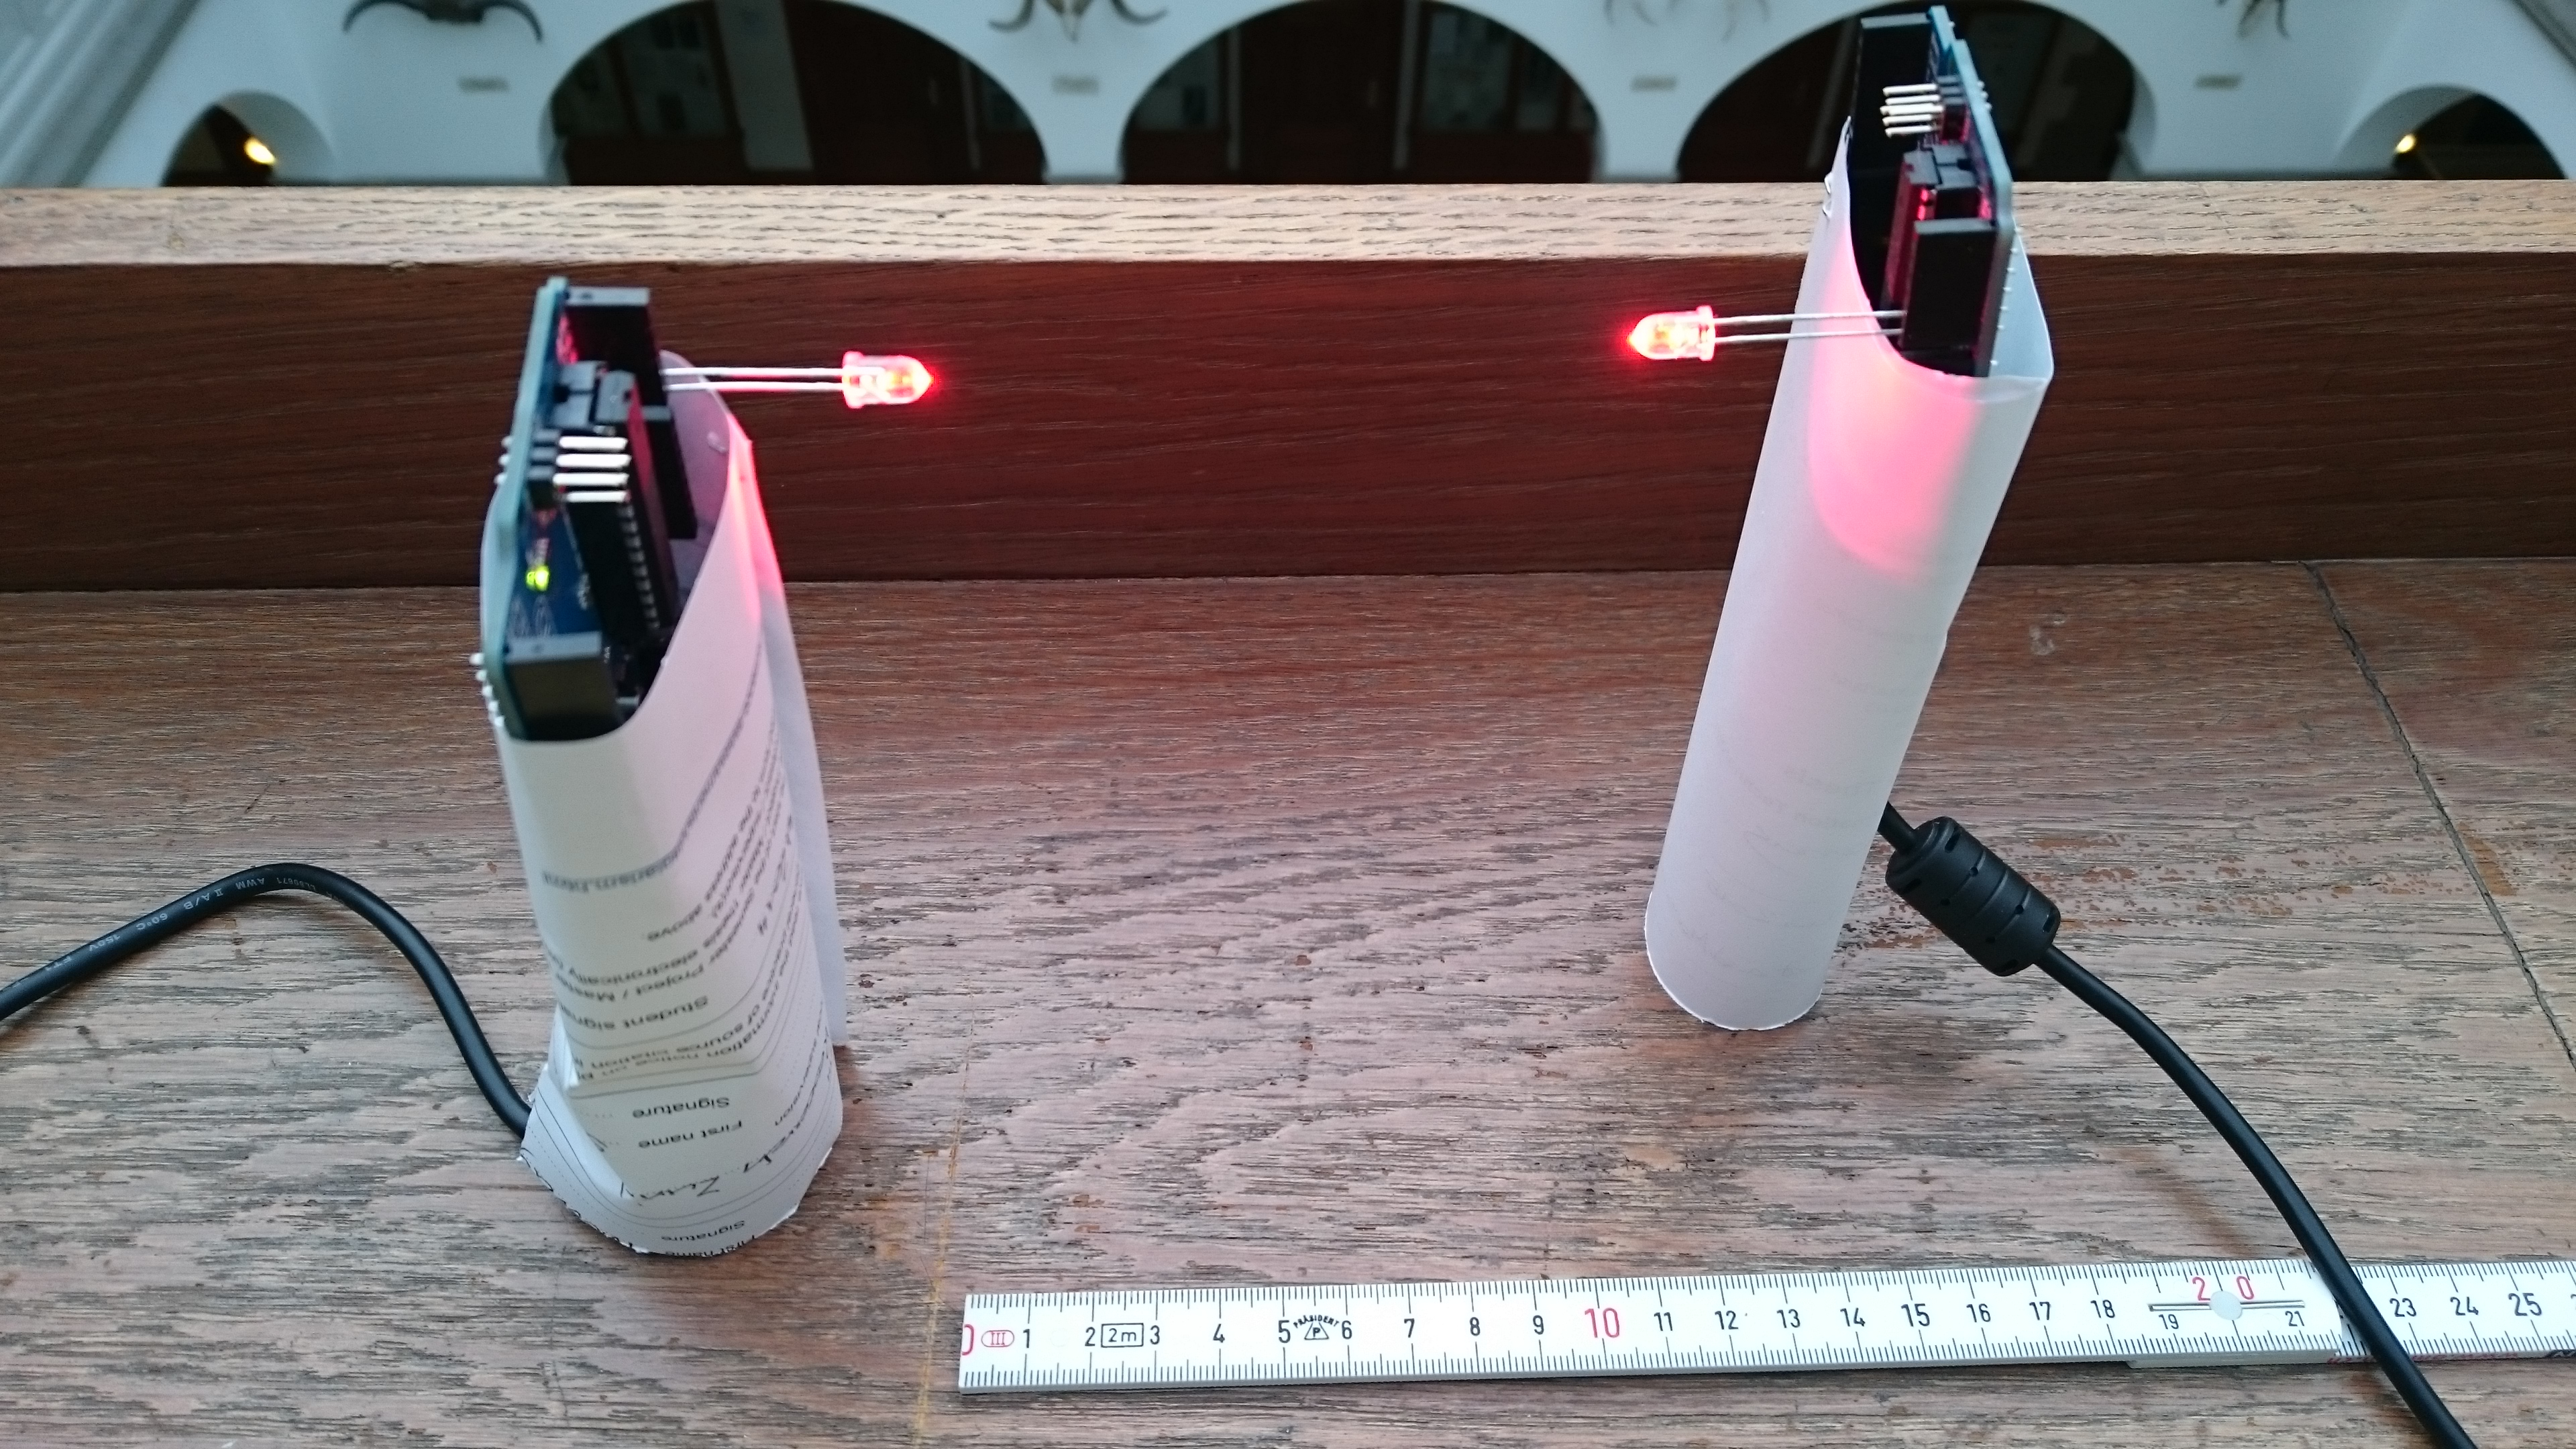
\includegraphics[width=\textwidth]{../img/setup_1.JPG}
\caption{}
\label{}
\end{figure}
\begin{figure}[htp]
\centering
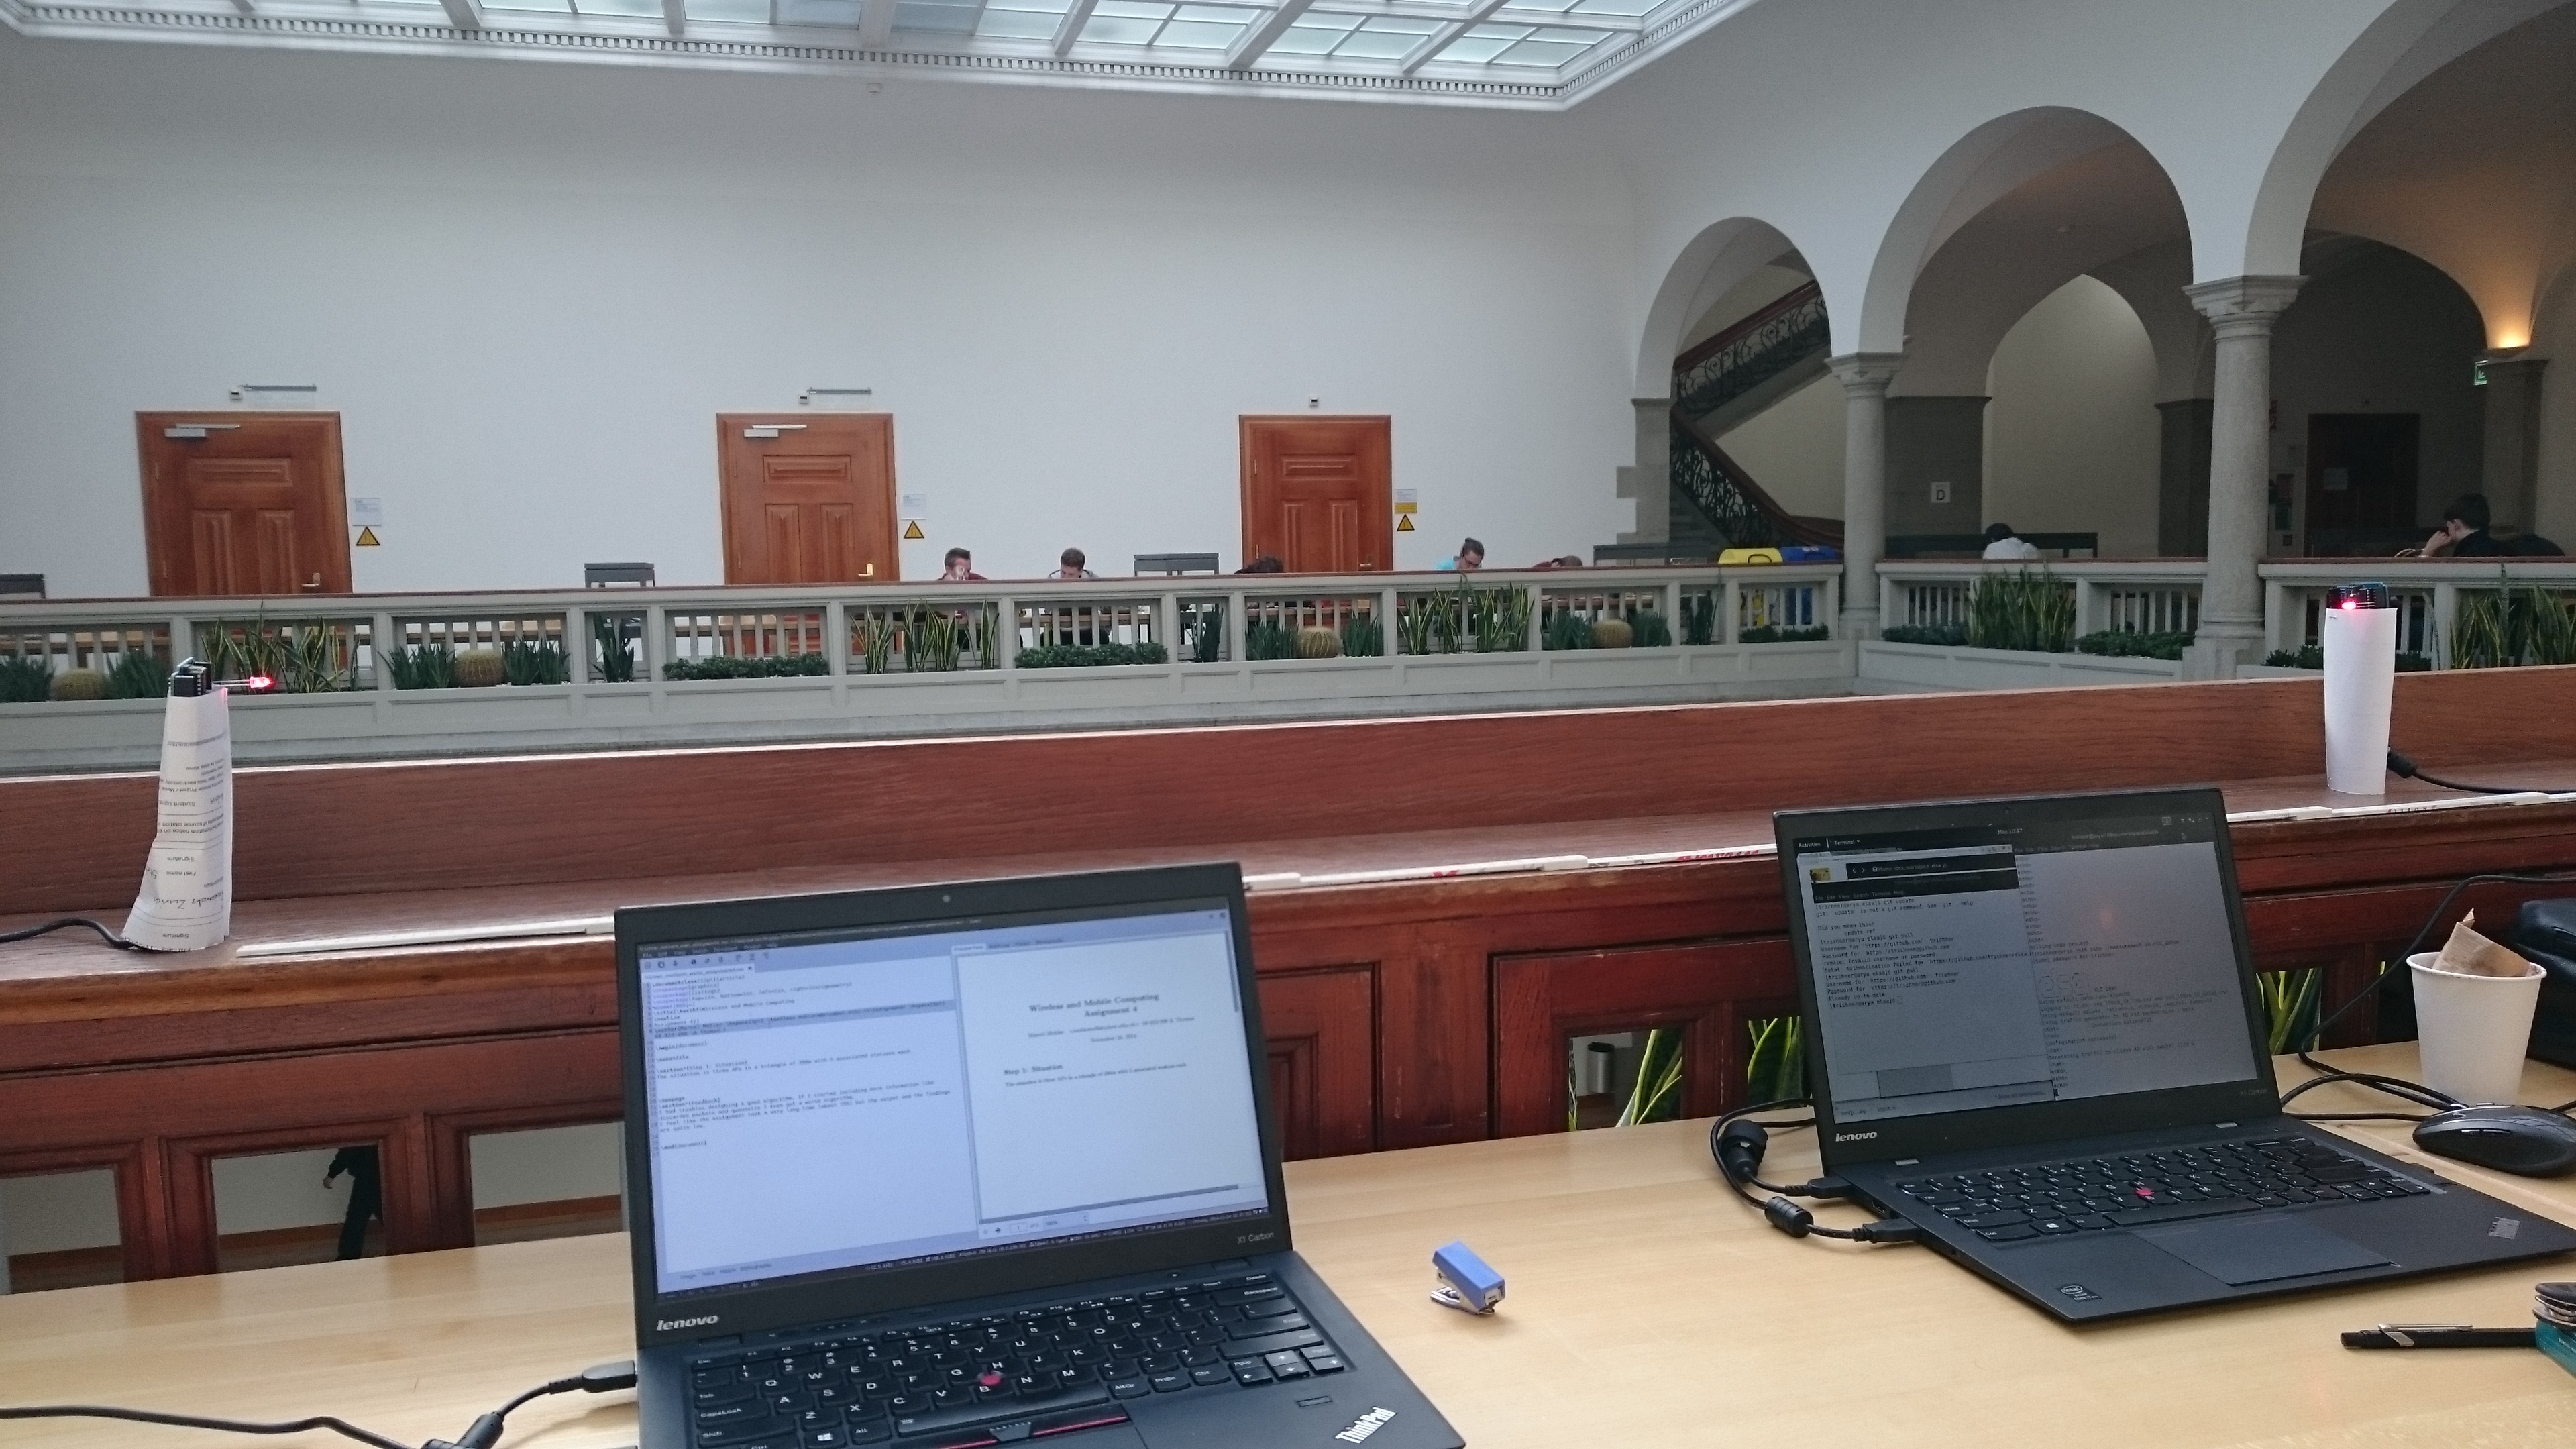
\includegraphics[width=\textwidth]{../img/setup_2.JPG}
\caption{}
\label{}
\end{figure}

\subsection{Setup}
We use short pylons to keep the two devices in the air in order to reduce effects from reflection on the ground.
Then we point the LEDs of both devices directly at each other and initialize one device as a receiver. The second device is configured to send as many packets as possible, meaning that it would send a new package as soon as the previous one was either ACK'ed or discarded.

We made measurements for the following distances: 10cm, 20cm, 50cm, 70cm, 100cm, 110cm, 120cm, 150cm and 200cm. For every distance we measured the throughput and delay for multiple different package sizes, which are 1B, 10B, 20B, 50B, 100B, 150B and 197B (Configuration values higher than this seemed to always fail, therefore we approximated 200B with 197B). Every measurement series was taken over an interval of 60s.


\subsection{Results}
In Figure \ref{fig:chanchar} one can clearly see that the maximum successful transmission distance is at 110m in our case. For distances greater than 110cm we could not transmit any data successfully i.e. we never received an ACK for data sent, nevertheless the receiver managed to receive at least partial packets.
The diagram also shows that there is a clear tradeoff between throughput and delay by choosing a packetsize. Bigger packetsizes result in higher throughput while also increasing the delay.

The upper and lower value of the 90\% confidence interval for the delay differ in less than one millisecond in all our measurements, whereas our setups time resolution is at most one millisecond. Hence we do not try to display it in the (already crowded) diagram.




\begin{figure}[htp]
\centering
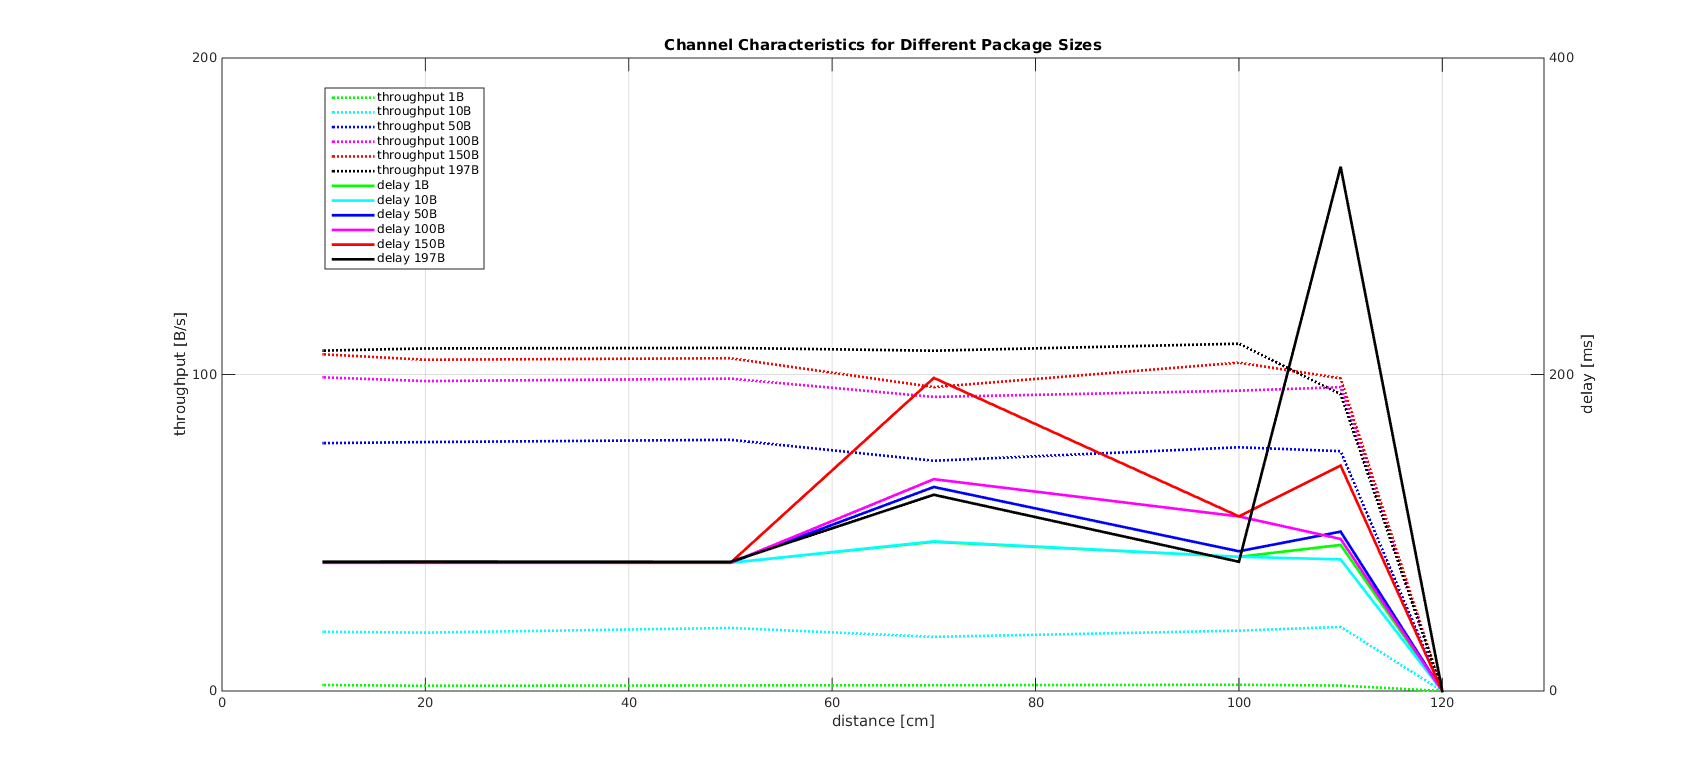
\includegraphics[width=\textwidth]{../img/plot_channel-characteristics.png}
\caption{VLC channel characteristics for differing package sizes and distances}
\label{fig:chanchar}
\end{figure}

The following table shows the standard deviation of the delay for all measurement series, note  that it is below one millisecond for combinations with small packetsizes and distances but can be in the order of hundreds of milliseconds for the bigger packetsizes and higher distances.

\begin{verbatim}
    packetsize    distance     stddev 
    __________    ________    ________

      1            10          0.27059
      1            20          0.15107
      1            50          0.11951
      1            70            52.27
      1           100           26.046
      1           110           46.795
      1           120                0
     10            10          0.40089
     10            20          0.15171
     10            50          0.21592
     10            70           52.601
     10           100           29.474
     10           110           21.443
     10           120                0
     50            10          0.41783
     50            20         0.089087
     50            50          0.29479
     50            70           156.31
     50           100           58.619
     50           110           97.642
     50           120                0
    100            10          0.12127
    100            20                0
    100            50                0
    100            70           208.96
    100           100           168.37
    100           110           121.55
    100           120                0
    150            10          0.37129
    150            20          0.37498
    150            50          0.14744
    150            70           464.99
    150           100           201.29
    150           110           284.91
    150           120                0
    197            10          0.46718
    197            20          0.42164
    197            50          0.49167
    197            70           253.54
    197           100          0.47458
    197           110           706.83
    197           120                0
\end{verbatim}